\newpage

\section{Saliency Analysis} \label{app:saliency}

This appendix provides comprehensive evaluation results for all XAI methods tested in the experimental setup described in \cref{subsec:eval_framework}.

\subsection{VGG16 Qualitative Saliency Map Comparison} \label{app:vgg_qualitative}

Complementing \cref{fig:vgg_saliency_comparison_main}, we give more saliency examples in \cref{fig:vgg_saliency_comparison}. Again, we observe more focus on the whole classified objects by SplitCAM in layer 26 compared to LayerCAM in the same layer.
SplitGrad in layer 0 detects too many edges of the original image to be a useful explanation of the model's decision. Especially in images with many image details in the background, \eg the rubble in the wood rabbit image, it fails to focus on the important image parts. 
This aligns with the observed performance peaks of SplitGrad and SplitCAM in deeper layers, presented in \cref{fig:layer_dependence} in the layer ablation studies.

\begin{figure}[H]
    \centering

    \begin{minipage}[c]{0.08\linewidth}
        \centering
        \scriptsize \textbf{Class}
    \end{minipage}\hspace{0.002\linewidth}%
    \begin{minipage}[c]{0.10\linewidth}
        \centering
        \scriptsize \textbf{Original}
    \end{minipage}\hspace{0.002\linewidth}%
    \begin{minipage}[c]{0.10\linewidth}
        \centering
        \scriptsize \textbf{SplitLRP}\\
        \scriptsize \textbf{(10, pos) abs}
    \end{minipage}\hspace{0.002\linewidth}%
    \begin{minipage}[c]{0.10\linewidth}
        \centering
        \scriptsize \textbf{LRP $\gamma$=0.25}\\
        \scriptsize \textbf{layer 5 abs}
    \end{minipage}\hspace{0.002\linewidth}%
    \begin{minipage}[c]{0.10\linewidth}
        \centering
        \scriptsize \textbf{SplitCAM}\\
        \scriptsize \textbf{(14, g) $\alpha=0.4$}
    \end{minipage}\hspace{0.002\linewidth}%
    \begin{minipage}[c]{0.10\linewidth}
        \centering
        \scriptsize \textbf{LayerCAM}\\
        \scriptsize \textbf{layer 14}
    \end{minipage}\hspace{0.002\linewidth}%
    \begin{minipage}[c]{0.10\linewidth}
        \centering
        \scriptsize \textbf{SplitCAM}\\
        \scriptsize \textbf{(26, g) $\alpha=0.3$ abs}
    \end{minipage}\hspace{0.002\linewidth}%
    \begin{minipage}[c]{0.10\linewidth}
        \centering
        \scriptsize \textbf{LayerCAM}\\
        \scriptsize \textbf{layer 26}
    \end{minipage}\hspace{0.002\linewidth}%
    \begin{minipage}[c]{0.10\linewidth}
        \centering
        \scriptsize \textbf{SplitGrad}\\
        \scriptsize \textbf{(0, +, g)}
    \end{minipage}

    \vspace{0.3cm}

    \begin{minipage}[c]{0.08\linewidth}
        \centering
        \small tiger shark\\[1pt]
        {\scriptsize (0.9979)}
    \end{minipage}\hspace{0.002\linewidth}%
    \begin{minipage}[c]{0.10\linewidth}
        \centering
        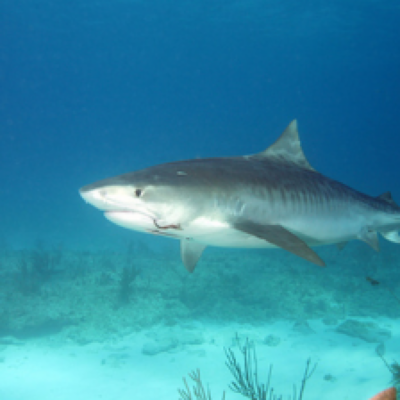
\includegraphics[width=\linewidth]{saliency_quality/image_0018_ILSVRC2012_val_00034038.JPEG/original_image.png}
    \end{minipage}\hspace{0.002\linewidth}%
    \begin{minipage}[c]{0.10\linewidth}
        \centering
        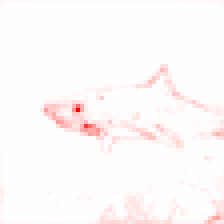
\includegraphics[width=\linewidth]{saliency_quality/image_0018_ILSVRC2012_val_00034038.JPEG/hybrid_lrp_scaling_max_winnerTakesItAllMaxpool_f10_cam_pp_abs.png}
    \end{minipage}\hspace{0.002\linewidth}%
    \begin{minipage}[c]{0.10\linewidth}
        \centering
        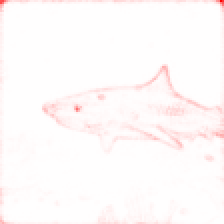
\includegraphics[width=\linewidth]{saliency_quality/image_0018_ILSVRC2012_val_00034038.JPEG/zennit_lrp_gamma0.25_features_5_abs.png}
    \end{minipage}\hspace{0.002\linewidth}%
    \begin{minipage}[c]{0.10\linewidth}
        \centering
        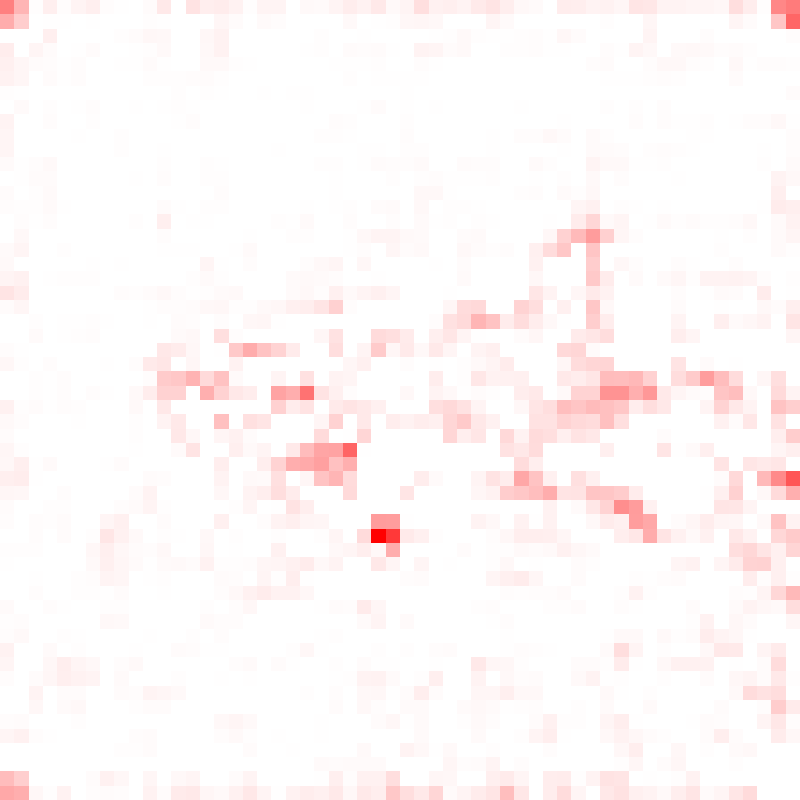
\includegraphics[width=\linewidth]{saliency_quality/image_0018_ILSVRC2012_val_00034038.JPEG/hybrid_cam_shift_40_scale_max_winnerTakesItAllMaxpool_f14_cam_g.png}
    \end{minipage}\hspace{0.002\linewidth}%
    \begin{minipage}[c]{0.10\linewidth}
        \centering
        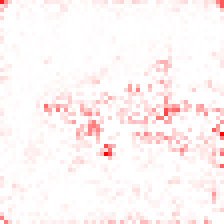
\includegraphics[width=\linewidth]{saliency_quality/image_0018_ILSVRC2012_val_00034038.JPEG/layer_cam_features_14_relu.png}
    \end{minipage}\hspace{0.002\linewidth}%
    \begin{minipage}[c]{0.10\linewidth}
        \centering
        
\includegraphics[width=\linewidth]{saliency_quality/image_0018_ILSVRC2012_val_00034038.JPEG/hybrid_cam_shift_30_scale_max_winnerTakesItAllMaxpool_f26_cam_g_abs.png}
    \end{minipage}\hspace{0.002\linewidth}%
    \begin{minipage}[c]{0.10\linewidth}
        \centering
        
\includegraphics[width=\linewidth]{saliency_quality/image_0018_ILSVRC2012_val_00034038.JPEG/layer_cam_features_26_relu.png}
    \end{minipage}\hspace{0.002\linewidth}%
    \begin{minipage}[c]{0.10\linewidth}
        \centering
        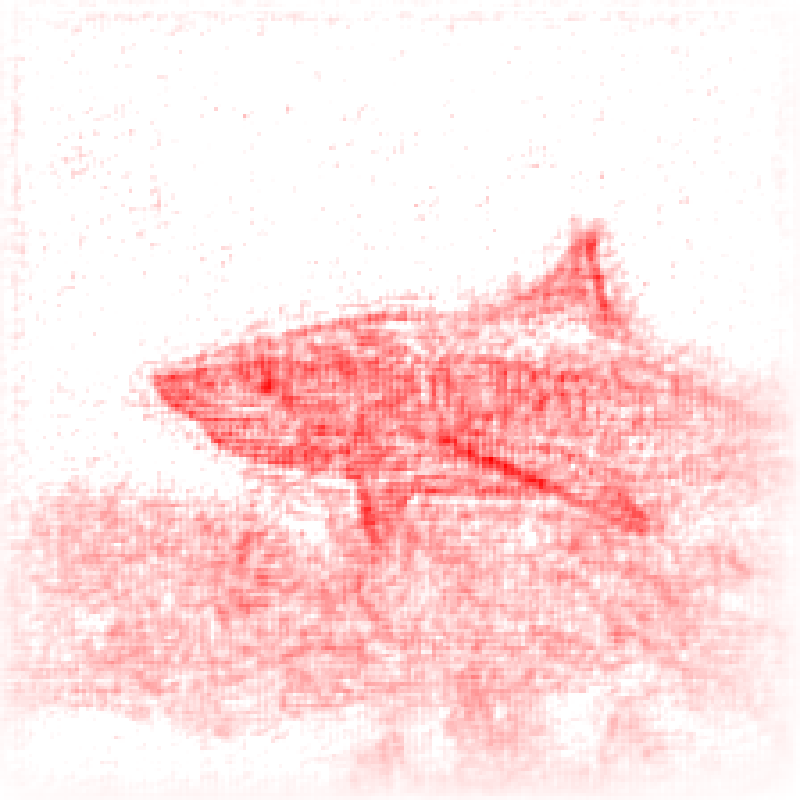
\includegraphics[width=\linewidth]{saliency_quality/image_0018_ILSVRC2012_val_00034038.JPEG/hybrid_grad_shift_30_max_winnerTakesItAllMaxpool_f0_grad_pp.png}
    \end{minipage}%

    \vspace{0.3cm}

    \begin{minipage}[c]{0.08\linewidth}
        \centering
        \small goldfinch\\[1pt]
        {\scriptsize (1.0000)}
    \end{minipage}\hspace{0.002\linewidth}%
    \begin{minipage}[c]{0.10\linewidth}
        \centering
        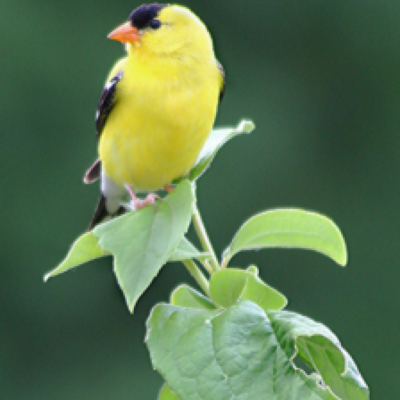
\includegraphics[width=\linewidth]{saliency_quality/image_0034_ILSVRC2012_val_00044706.JPEG/original_image.png}
    \end{minipage}\hspace{0.002\linewidth}%
    \begin{minipage}[c]{0.10\linewidth}
        \centering
        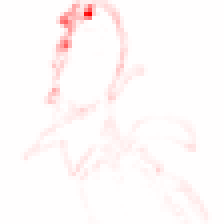
\includegraphics[width=\linewidth]{saliency_quality/image_0034_ILSVRC2012_val_00044706.JPEG/hybrid_lrp_scaling_max_winnerTakesItAllMaxpool_f10_cam_pp_abs.png}
    \end{minipage}\hspace{0.002\linewidth}%
    \begin{minipage}[c]{0.10\linewidth}
        \centering
        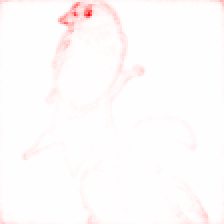
\includegraphics[width=\linewidth]{saliency_quality/image_0034_ILSVRC2012_val_00044706.JPEG/zennit_lrp_gamma0.25_features_5_abs.png}
    \end{minipage}\hspace{0.002\linewidth}%
    \begin{minipage}[c]{0.10\linewidth}
        \centering
        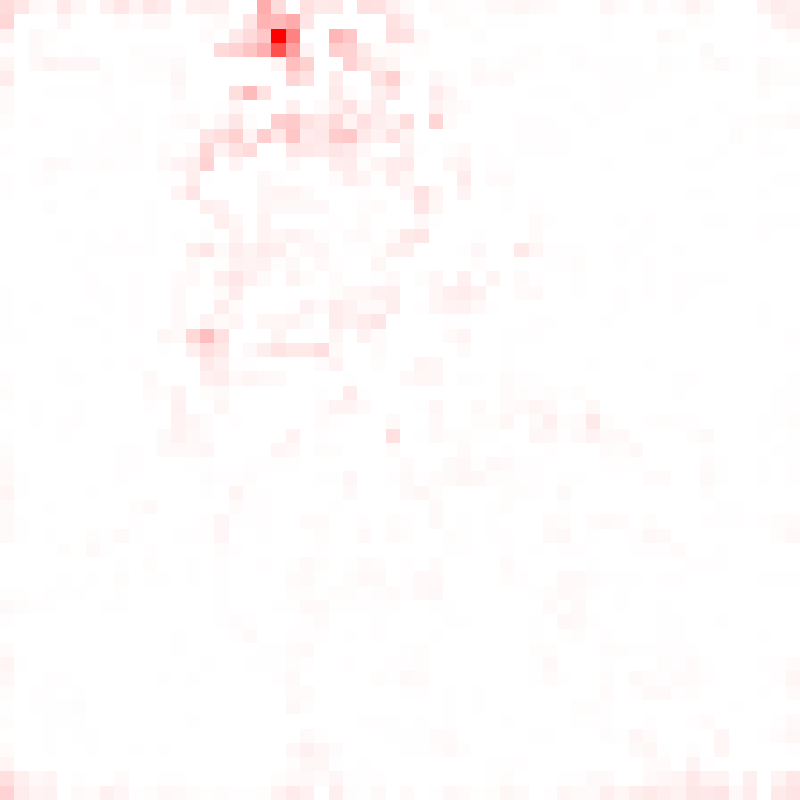
\includegraphics[width=\linewidth]{saliency_quality/image_0034_ILSVRC2012_val_00044706.JPEG/hybrid_cam_shift_40_scale_max_winnerTakesItAllMaxpool_f14_cam_g.png}
    \end{minipage}\hspace{0.002\linewidth}%
    \begin{minipage}[c]{0.10\linewidth}
        \centering
        
\includegraphics[width=\linewidth]{saliency_quality/image_0034_ILSVRC2012_val_00044706.JPEG/layer_cam_features_14_relu.png}
    \end{minipage}\hspace{0.002\linewidth}%
    \begin{minipage}[c]{0.10\linewidth}
        \centering
        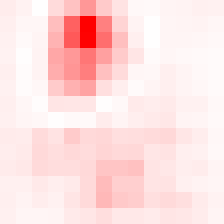
\includegraphics[width=\linewidth]{saliency_quality/image_0034_ILSVRC2012_val_00044706.JPEG/hybrid_cam_shift_30_scale_max_winnerTakesItAllMaxpool_f26_cam_g_abs.png}
    \end{minipage}\hspace{0.002\linewidth}%
    \begin{minipage}[c]{0.10\linewidth}
        \centering
        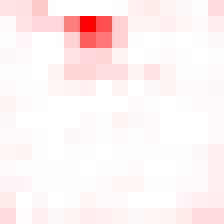
\includegraphics[width=\linewidth]{saliency_quality/image_0034_ILSVRC2012_val_00044706.JPEG/layer_cam_features_26_relu.png}
    \end{minipage}\hspace{0.002\linewidth}%
    \begin{minipage}[c]{0.10\linewidth}
        \centering
        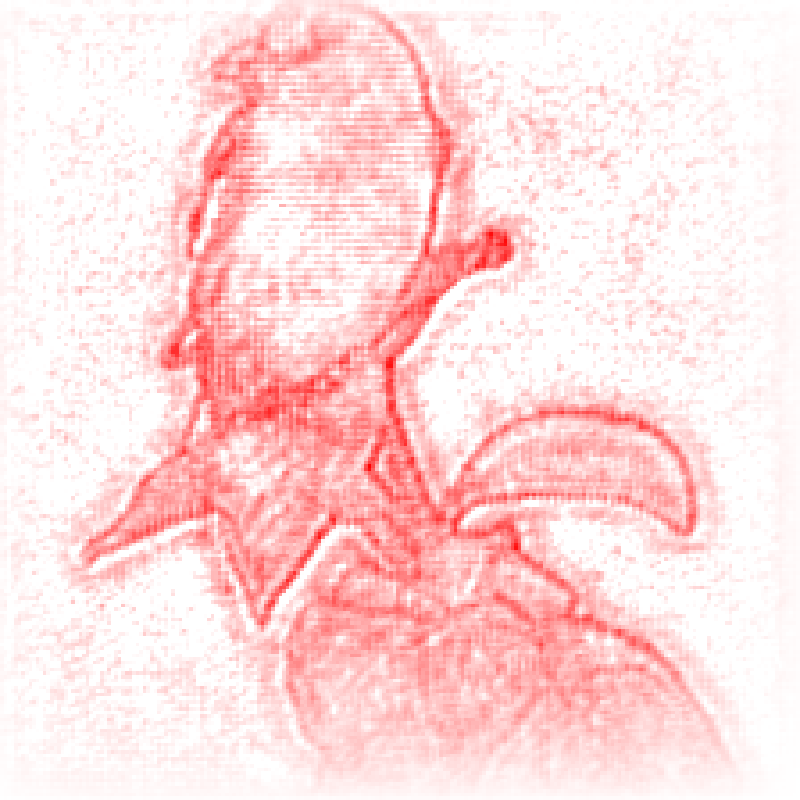
\includegraphics[width=\linewidth]{saliency_quality/image_0034_ILSVRC2012_val_00044706.JPEG/hybrid_grad_shift_30_max_winnerTakesItAllMaxpool_f0_grad_pp.png}
    \end{minipage}%

    \vspace{0.3cm}

    \begin{minipage}[c]{0.08\linewidth}
        \centering
        \small tree frog\\[1pt]
        {\scriptsize (0.9954)}
    \end{minipage}\hspace{0.002\linewidth}%
    \begin{minipage}[c]{0.10\linewidth}
        \centering
        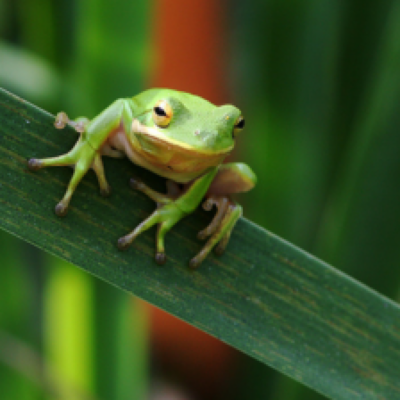
\includegraphics[width=\linewidth]{saliency_quality/image_0041_ILSVRC2012_val_00017505.JPEG/original_image.png}
    \end{minipage}\hspace{0.002\linewidth}%
    \begin{minipage}[c]{0.10\linewidth}
        \centering
        
\includegraphics[width=\linewidth]{saliency_quality/image_0041_ILSVRC2012_val_00017505.JPEG/hybrid_lrp_scaling_max_winnerTakesItAllMaxpool_f10_cam_pp_abs.png}
    \end{minipage}\hspace{0.002\linewidth}%
    \begin{minipage}[c]{0.10\linewidth}
        \centering
        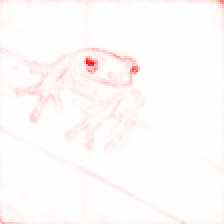
\includegraphics[width=\linewidth]{saliency_quality/image_0041_ILSVRC2012_val_00017505.JPEG/zennit_lrp_gamma0.25_features_5_abs.png}
    \end{minipage}\hspace{0.002\linewidth}%
    \begin{minipage}[c]{0.10\linewidth}
        \centering
        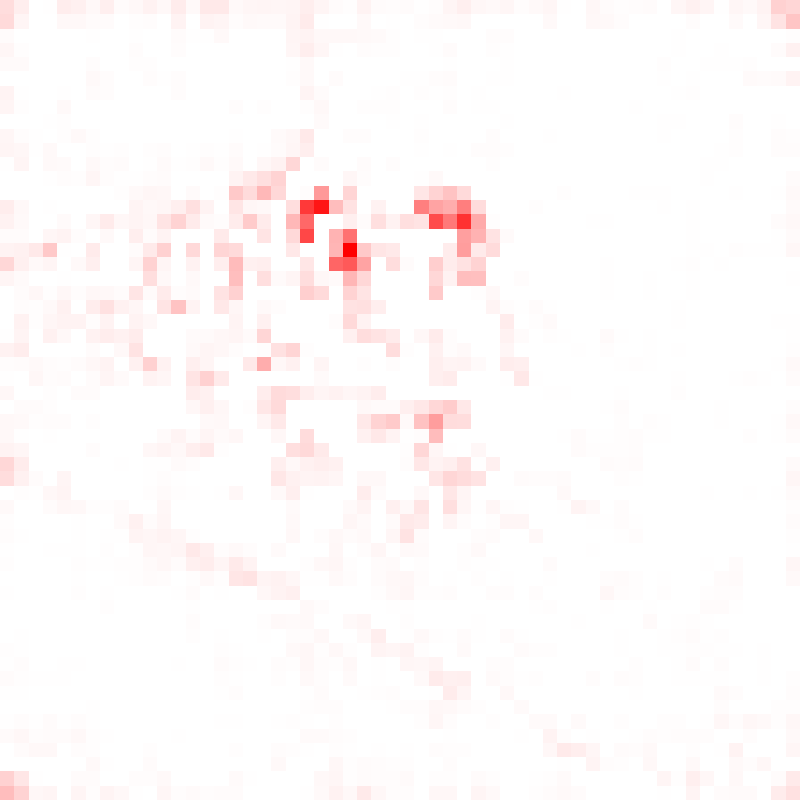
\includegraphics[width=\linewidth]{saliency_quality/image_0041_ILSVRC2012_val_00017505.JPEG/hybrid_cam_shift_40_scale_max_winnerTakesItAllMaxpool_f14_cam_g.png}
    \end{minipage}\hspace{0.002\linewidth}%
    \begin{minipage}[c]{0.10\linewidth}
        \centering
        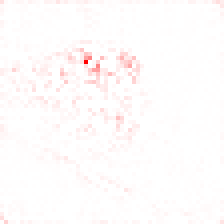
\includegraphics[width=\linewidth]{saliency_quality/image_0041_ILSVRC2012_val_00017505.JPEG/layer_cam_features_14_relu.png}
    \end{minipage}\hspace{0.002\linewidth}%
    \begin{minipage}[c]{0.10\linewidth}
        \centering
        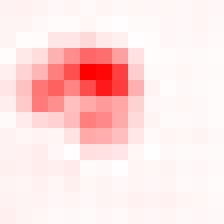
\includegraphics[width=\linewidth]{saliency_quality/image_0041_ILSVRC2012_val_00017505.JPEG/hybrid_cam_shift_30_scale_max_winnerTakesItAllMaxpool_f26_cam_g_abs.png}
    \end{minipage}\hspace{0.002\linewidth}%
    \begin{minipage}[c]{0.10\linewidth}
        \centering
        
\includegraphics[width=\linewidth]{saliency_quality/image_0041_ILSVRC2012_val_00017505.JPEG/layer_cam_features_26_relu.png}
    \end{minipage}\hspace{0.002\linewidth}%
    \begin{minipage}[c]{0.10\linewidth}
        \centering
        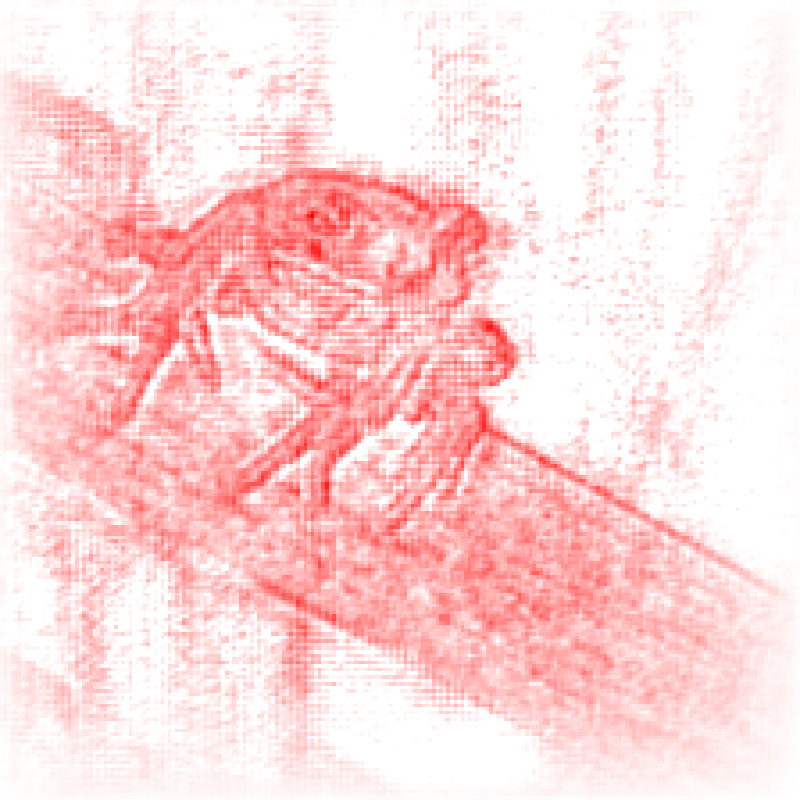
\includegraphics[width=\linewidth]{saliency_quality/image_0041_ILSVRC2012_val_00017505.JPEG/hybrid_grad_shift_30_max_winnerTakesItAllMaxpool_f0_grad_pp.png}
    \end{minipage}%

    \vspace{0.3cm}

    \begin{minipage}[c]{0.08\linewidth}
        \centering
        \small ladybug\\[1pt]
        {\scriptsize (0.8272)}
    \end{minipage}\hspace{0.002\linewidth}%
    \begin{minipage}[c]{0.10\linewidth}
        \centering
        
\includegraphics[width=\linewidth]{saliency_quality/image_0096_ILSVRC2012_val_00025218.JPEG/original_image.png}
    \end{minipage}\hspace{0.002\linewidth}%
    \begin{minipage}[c]{0.10\linewidth}
        \centering
        
\includegraphics[width=\linewidth]{saliency_quality/image_0096_ILSVRC2012_val_00025218.JPEG/hybrid_lrp_scaling_max_winnerTakesItAllMaxpool_f10_cam_pp_abs.png}
    \end{minipage}\hspace{0.002\linewidth}%
    \begin{minipage}[c]{0.10\linewidth}
        \centering
        
\includegraphics[width=\linewidth]{saliency_quality/image_0096_ILSVRC2012_val_00025218.JPEG/zennit_lrp_gamma0.25_features_5_abs.png}
    \end{minipage}\hspace{0.002\linewidth}%
    \begin{minipage}[c]{0.10\linewidth}
        \centering
        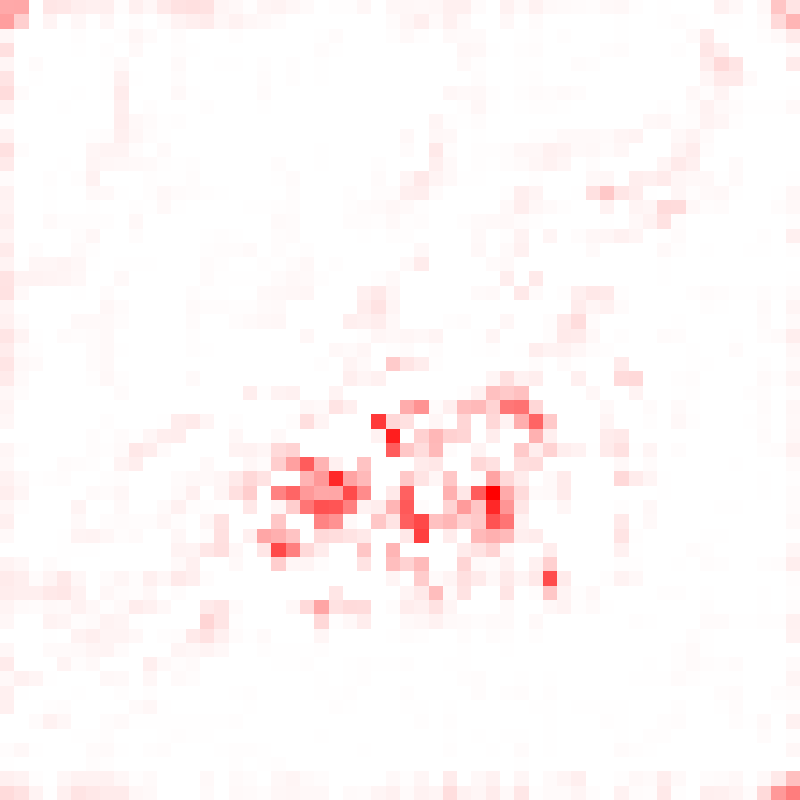
\includegraphics[width=\linewidth]{saliency_quality/image_0096_ILSVRC2012_val_00025218.JPEG/hybrid_cam_shift_40_scale_max_winnerTakesItAllMaxpool_f14_cam_g.png}
    \end{minipage}\hspace{0.002\linewidth}%
    \begin{minipage}[c]{0.10\linewidth}
        \centering
        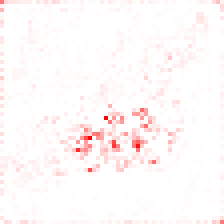
\includegraphics[width=\linewidth]{saliency_quality/image_0096_ILSVRC2012_val_00025218.JPEG/layer_cam_features_14_relu.png}
    \end{minipage}\hspace{0.002\linewidth}%
    \begin{minipage}[c]{0.10\linewidth}
        \centering
        
\includegraphics[width=\linewidth]{saliency_quality/image_0096_ILSVRC2012_val_00025218.JPEG/hybrid_cam_shift_30_scale_max_winnerTakesItAllMaxpool_f26_cam_g_abs.png}
    \end{minipage}\hspace{0.002\linewidth}%
    \begin{minipage}[c]{0.10\linewidth}
        \centering
        
\includegraphics[width=\linewidth]{saliency_quality/image_0096_ILSVRC2012_val_00025218.JPEG/layer_cam_features_26_relu.png}
    \end{minipage}\hspace{0.002\linewidth}%
    \begin{minipage}[c]{0.10\linewidth}
        \centering
        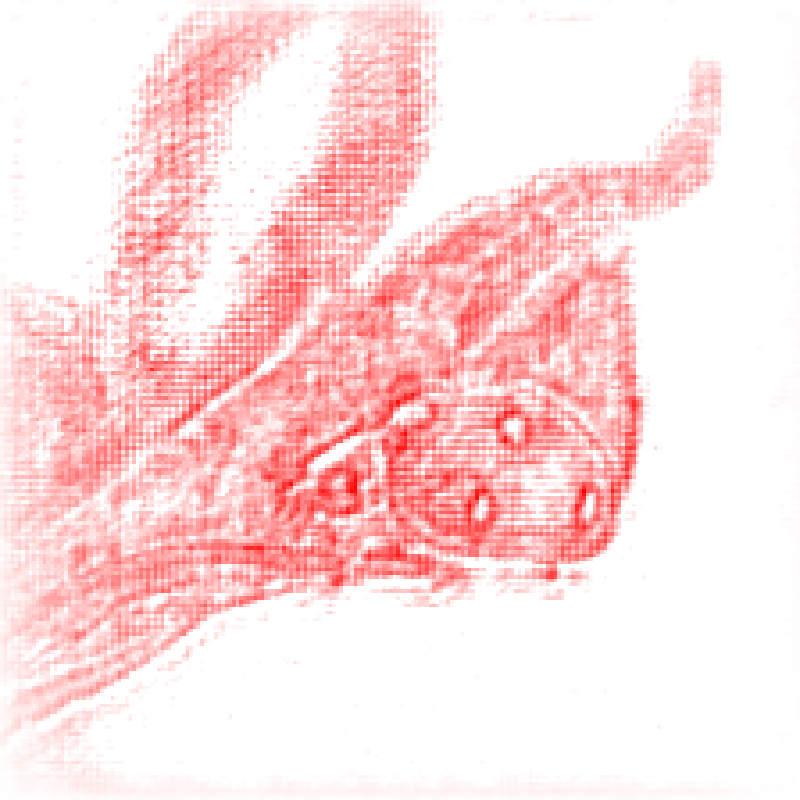
\includegraphics[width=\linewidth]{saliency_quality/image_0096_ILSVRC2012_val_00025218.JPEG/hybrid_grad_shift_30_max_winnerTakesItAllMaxpool_f0_grad_pp.png}
    \end{minipage}%

    \vspace{0.3cm}

    \begin{minipage}[c]{0.08\linewidth}
        \centering
        \small wood rabbit\\[1pt]
        {\scriptsize (0.9782)}
    \end{minipage}\hspace{0.002\linewidth}%
    \begin{minipage}[c]{0.10\linewidth}
        \centering
        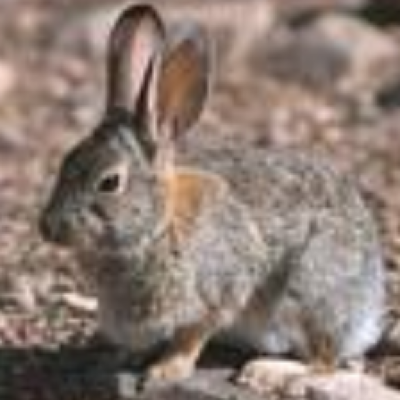
\includegraphics[width=\linewidth]{saliency_quality/image_0120_ILSVRC2012_val_00024858.JPEG/original_image.png}
    \end{minipage}\hspace{0.002\linewidth}%
    \begin{minipage}[c]{0.10\linewidth}
        \centering
        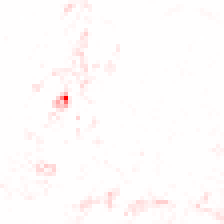
\includegraphics[width=\linewidth]{saliency_quality/image_0120_ILSVRC2012_val_00024858.JPEG/hybrid_lrp_scaling_max_winnerTakesItAllMaxpool_f10_cam_pp_abs.png}
    \end{minipage}\hspace{0.002\linewidth}%
    \begin{minipage}[c]{0.10\linewidth}
        \centering
        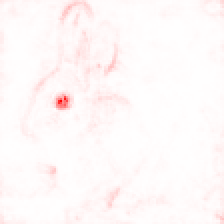
\includegraphics[width=\linewidth]{saliency_quality/image_0120_ILSVRC2012_val_00024858.JPEG/zennit_lrp_gamma0.25_features_5_abs.png}
    \end{minipage}\hspace{0.002\linewidth}%
    \begin{minipage}[c]{0.10\linewidth}
        \centering
        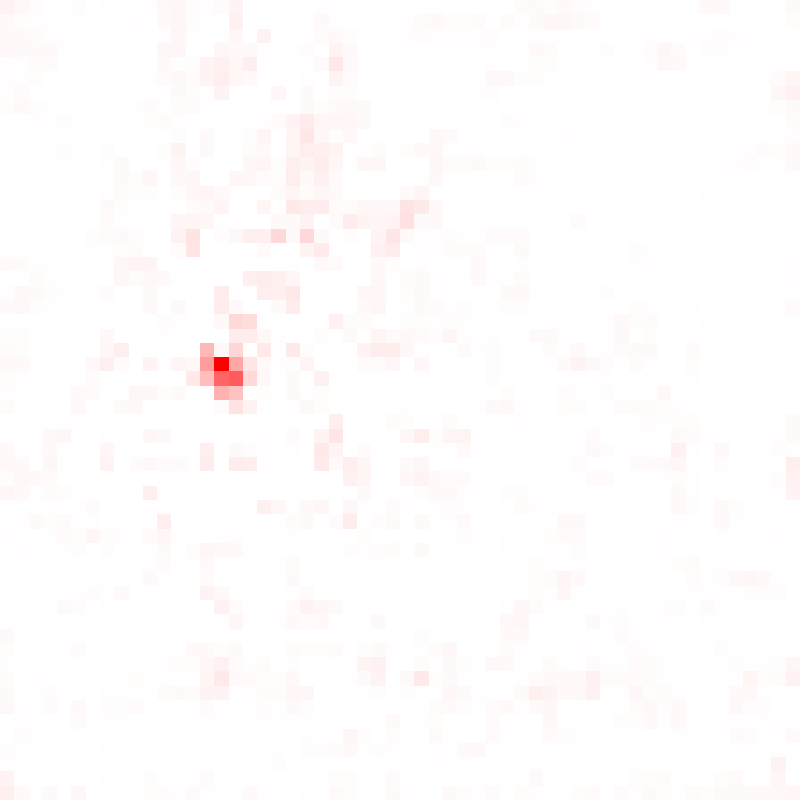
\includegraphics[width=\linewidth]{saliency_quality/image_0120_ILSVRC2012_val_00024858.JPEG/hybrid_cam_shift_40_scale_max_winnerTakesItAllMaxpool_f14_cam_g.png}
    \end{minipage}\hspace{0.002\linewidth}%
    \begin{minipage}[c]{0.10\linewidth}
        \centering
        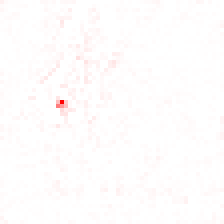
\includegraphics[width=\linewidth]{saliency_quality/image_0120_ILSVRC2012_val_00024858.JPEG/layer_cam_features_14_relu.png}
    \end{minipage}\hspace{0.002\linewidth}%
    \begin{minipage}[c]{0.10\linewidth}
        \centering
        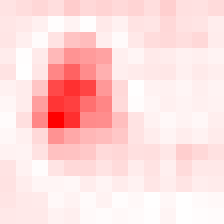
\includegraphics[width=\linewidth]{saliency_quality/image_0120_ILSVRC2012_val_00024858.JPEG/hybrid_cam_shift_30_scale_max_winnerTakesItAllMaxpool_f26_cam_g_abs.png}
    \end{minipage}\hspace{0.002\linewidth}%
    \begin{minipage}[c]{0.10\linewidth}
        \centering
        
\includegraphics[width=\linewidth]{saliency_quality/image_0120_ILSVRC2012_val_00024858.JPEG/layer_cam_features_26_relu.png}
    \end{minipage}\hspace{0.002\linewidth}%
    \begin{minipage}[c]{0.10\linewidth}
        \centering
        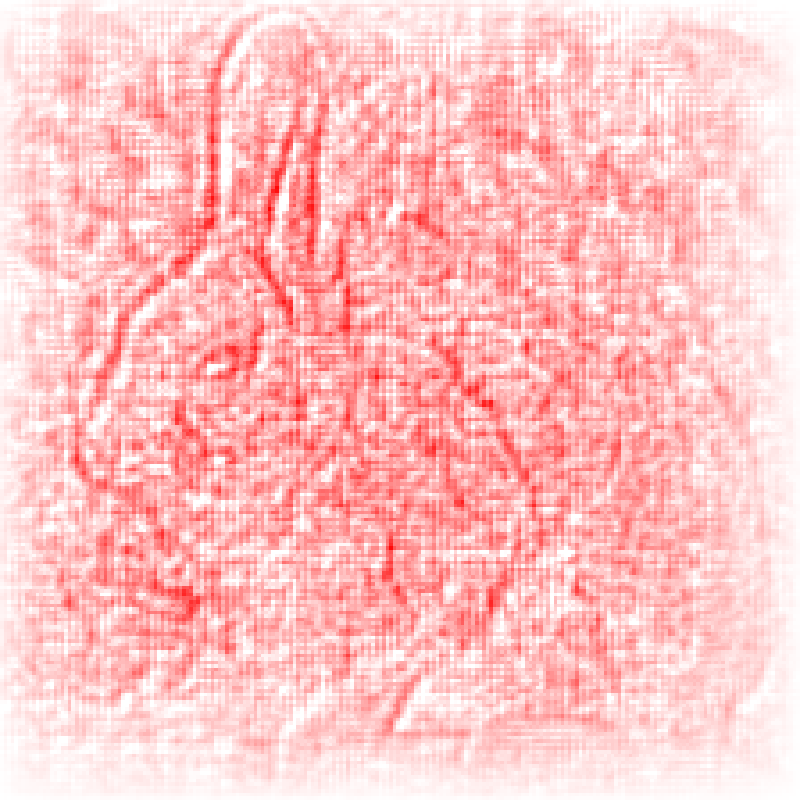
\includegraphics[width=\linewidth]{saliency_quality/image_0120_ILSVRC2012_val_00024858.JPEG/hybrid_grad_shift_30_max_winnerTakesItAllMaxpool_f0_grad_pp.png}
    \end{minipage}%

    \vspace{0.3cm}

    \begin{minipage}[c]{0.08\linewidth}
        \centering
        \small water tower\\[1pt]
        {\scriptsize (1.0000)}
    \end{minipage}\hspace{0.002\linewidth}%
    \begin{minipage}[c]{0.10\linewidth}
        \centering
        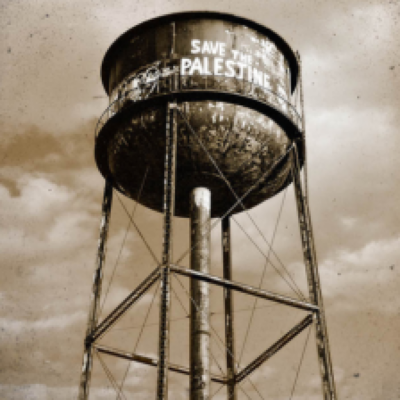
\includegraphics[width=\linewidth]{saliency_quality/image_0499_ILSVRC2012_val_00037082.JPEG/original_image.png}
    \end{minipage}\hspace{0.002\linewidth}%
    \begin{minipage}[c]{0.10\linewidth}
        \centering
        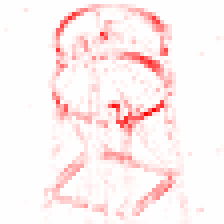
\includegraphics[width=\linewidth]{saliency_quality/image_0499_ILSVRC2012_val_00037082.JPEG/hybrid_lrp_scaling_max_winnerTakesItAllMaxpool_f10_cam_pp_abs.png}
    \end{minipage}\hspace{0.002\linewidth}%
    \begin{minipage}[c]{0.10\linewidth}
        \centering
        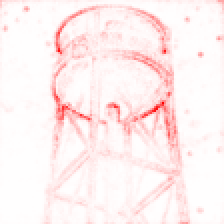
\includegraphics[width=\linewidth]{saliency_quality/image_0499_ILSVRC2012_val_00037082.JPEG/zennit_lrp_gamma0.25_features_5_abs.png}
    \end{minipage}\hspace{0.002\linewidth}%
    \begin{minipage}[c]{0.10\linewidth}
        \centering
        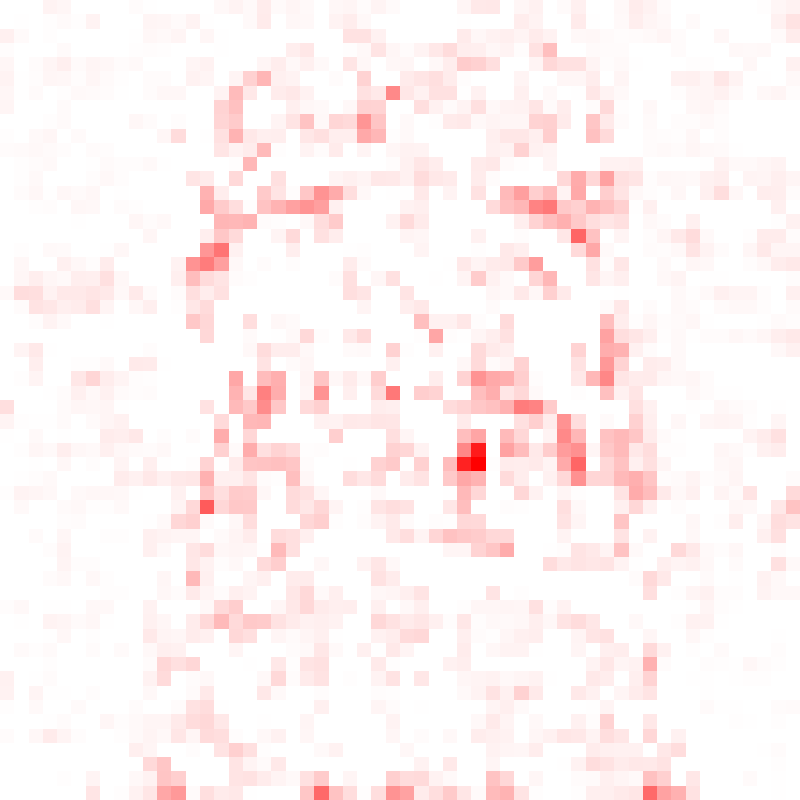
\includegraphics[width=\linewidth]{saliency_quality/image_0499_ILSVRC2012_val_00037082.JPEG/hybrid_cam_shift_40_scale_max_winnerTakesItAllMaxpool_f14_cam_g.png}
    \end{minipage}\hspace{0.002\linewidth}%
    \begin{minipage}[c]{0.10\linewidth}
        \centering
        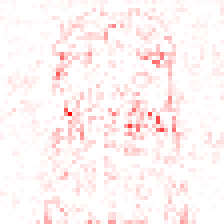
\includegraphics[width=\linewidth]{saliency_quality/image_0499_ILSVRC2012_val_00037082.JPEG/layer_cam_features_14_relu.png}
    \end{minipage}\hspace{0.002\linewidth}%
    \begin{minipage}[c]{0.10\linewidth}
        \centering
        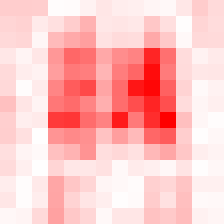
\includegraphics[width=\linewidth]{saliency_quality/image_0499_ILSVRC2012_val_00037082.JPEG/hybrid_cam_shift_30_scale_max_winnerTakesItAllMaxpool_f26_cam_g_abs.png}
    \end{minipage}\hspace{0.002\linewidth}%
    \begin{minipage}[c]{0.10\linewidth}
        \centering
        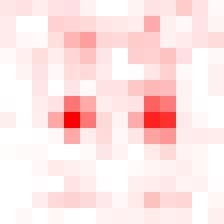
\includegraphics[width=\linewidth]{saliency_quality/image_0499_ILSVRC2012_val_00037082.JPEG/layer_cam_features_26_relu.png}
    \end{minipage}\hspace{0.002\linewidth}%
    \begin{minipage}[c]{0.10\linewidth}
        \centering
        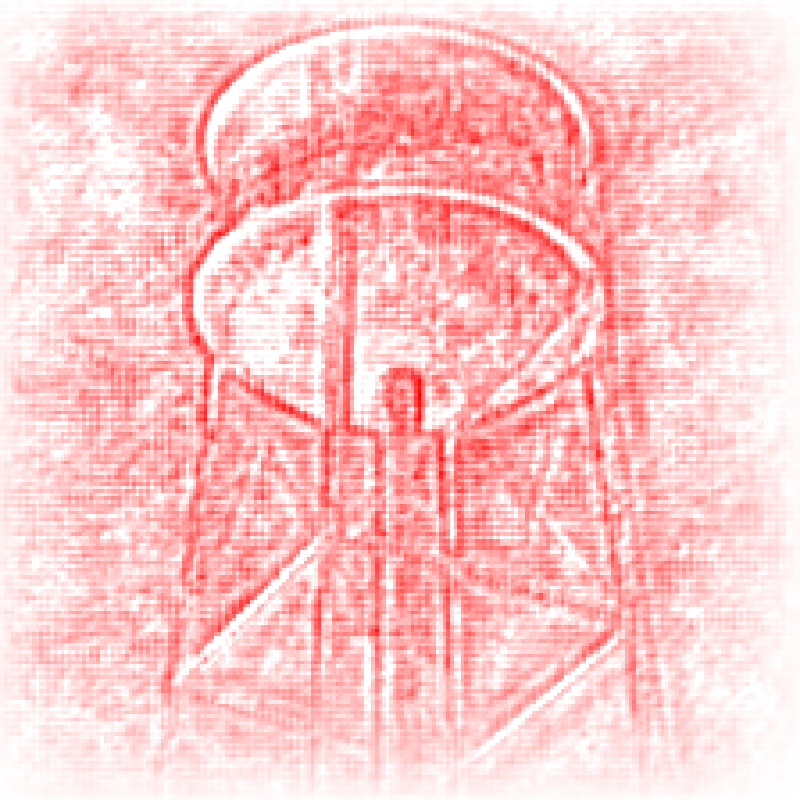
\includegraphics[width=\linewidth]{saliency_quality/image_0499_ILSVRC2012_val_00037082.JPEG/hybrid_grad_shift_30_max_winnerTakesItAllMaxpool_f0_grad_pp.png}
    \end{minipage}%

    \vspace{0.3cm}

    \begin{minipage}[c]{0.08\linewidth}
        \centering
        \small yawl\\[1pt]
        {\scriptsize (0.9953)}
    \end{minipage}\hspace{0.002\linewidth}%
    \begin{minipage}[c]{0.10\linewidth}
        \centering
        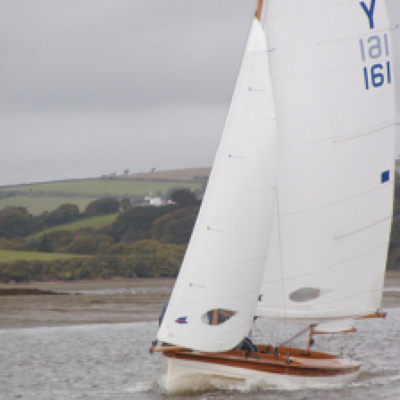
\includegraphics[width=\linewidth]{saliency_quality/image_0511_ILSVRC2012_val_00035734.JPEG/original_image.png}
    \end{minipage}\hspace{0.002\linewidth}%
    \begin{minipage}[c]{0.10\linewidth}
        \centering
        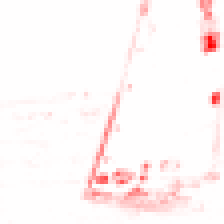
\includegraphics[width=\linewidth]{saliency_quality/image_0511_ILSVRC2012_val_00035734.JPEG/hybrid_lrp_scaling_max_winnerTakesItAllMaxpool_f10_cam_pp_abs.png}
    \end{minipage}\hspace{0.002\linewidth}%
    \begin{minipage}[c]{0.10\linewidth}
        \centering
        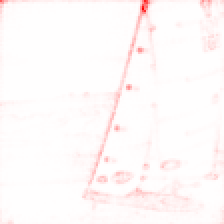
\includegraphics[width=\linewidth]{saliency_quality/image_0511_ILSVRC2012_val_00035734.JPEG/zennit_lrp_gamma0.25_features_5_abs.png}
    \end{minipage}\hspace{0.002\linewidth}%
    \begin{minipage}[c]{0.10\linewidth}
        \centering
        
\includegraphics[width=\linewidth]{saliency_quality/image_0511_ILSVRC2012_val_00035734.JPEG/hybrid_cam_shift_40_scale_max_winnerTakesItAllMaxpool_f14_cam_g.png}
    \end{minipage}\hspace{0.002\linewidth}%
    \begin{minipage}[c]{0.10\linewidth}
        \centering
        
\includegraphics[width=\linewidth]{saliency_quality/image_0511_ILSVRC2012_val_00035734.JPEG/layer_cam_features_14_relu.png}
    \end{minipage}\hspace{0.002\linewidth}%
    \begin{minipage}[c]{0.10\linewidth}
        \centering
        
\includegraphics[width=\linewidth]{saliency_quality/image_0511_ILSVRC2012_val_00035734.JPEG/hybrid_cam_shift_30_scale_max_winnerTakesItAllMaxpool_f26_cam_g_abs.png}
    \end{minipage}\hspace{0.002\linewidth}%
    \begin{minipage}[c]{0.10\linewidth}
        \centering
        
\includegraphics[width=\linewidth]{saliency_quality/image_0511_ILSVRC2012_val_00035734.JPEG/layer_cam_features_26_relu.png}
    \end{minipage}\hspace{0.002\linewidth}%
    \begin{minipage}[c]{0.10\linewidth}
        \centering
        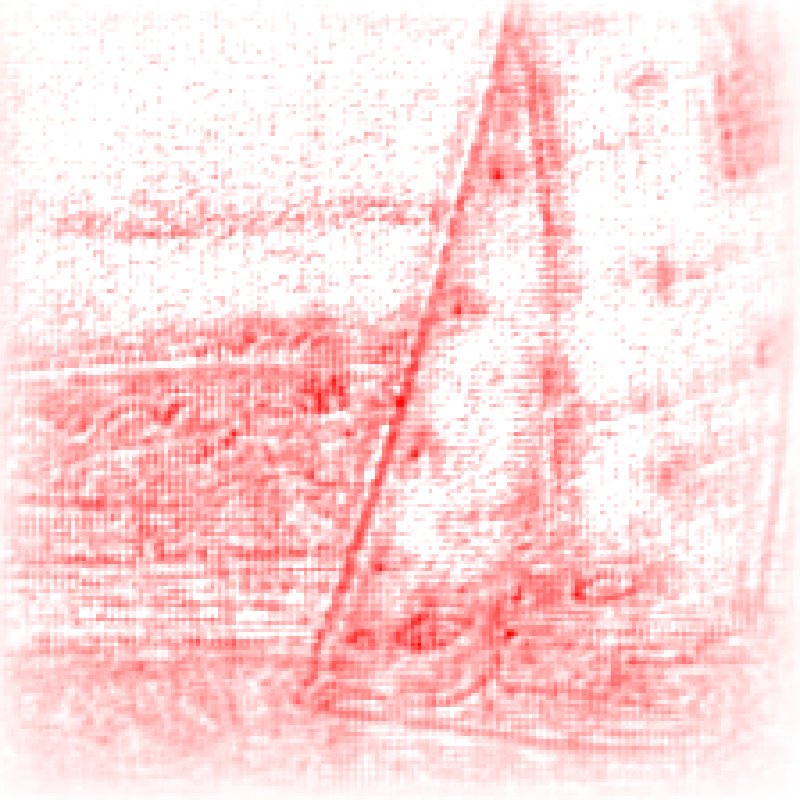
\includegraphics[width=\linewidth]{saliency_quality/image_0511_ILSVRC2012_val_00035734.JPEG/hybrid_grad_shift_30_max_winnerTakesItAllMaxpool_f0_grad_pp.png}
    \end{minipage}%

    \caption{Saliency map comparison for VGG16 on images from the custom ImageNet-S test subset. Each row shows the predicted class (with confidence), original image, and saliency maps from different methods. Methods include SplitLRP, classical LRP, SplitCAM variants, LayerCAM, and SplitGrad.}
    \label{fig:vgg_saliency_comparison}
\end{figure}


\newpage

\subsection{Quantitative Analysis on VGG16} \label{app:vgg_split}

\Cref{tab:xai_eval_comprehensive_vgg} presents detailed quantitative metrics analysis across all split configurations, baselines, and classical methods for VGG16. 
We observe a slight boost in performance between SplitCAM with $\alpha = 0.4$ compared to $\alpha = 0.5$ and compared to the classical LayerCAM respectively, indicating that the LayerCAM formulas indeed yield more powerful explanations on the split-pair compared to the original model. This can be seen even more drastically in ablation studies \cref{app:ablation}.

\begin{longtable}{p{4cm}|cc|cccccc}
    \caption{Comprehensive XAI Evaluation Results (VGG16). The abbreviations are similar to \cref{tab:eval_vgg_main}. 
    For each method configuration we highlight the best metrics values across the considered layer configurations in bold.}
    \label{tab:xai_eval_comprehensive_vgg} \\
    \toprule
    \textbf{Method} & \textbf{Layer} & \textbf{Abs} & \textbf{Select.} & \textbf{Attr. Loc.} & \textbf{Point.} & \textbf{Pixel Fl.} & \textbf{Pixel Fl.} & \textbf{Max Sens.} \\
     & & & \textbf{$\downarrow$} & \textbf{$\uparrow$} & \textbf{$\uparrow$} & \textbf{AUC@5 $\uparrow$} & \textbf{AUC@20 $\uparrow$} & \textbf{$\downarrow$} \\
    \midrule
    \endfirsthead
    
    \multicolumn{9}{c}%
    {{\tablename\ \thetable{} -- continued from previous page}} \\
    \toprule
    \textbf{Method} & \textbf{Layer} & \textbf{Abs} & \textbf{Select.} & \textbf{Attr. Loc.} & \textbf{Point.} & \textbf{Pixel Fl.} & \textbf{Pixel Fl.} & \textbf{Max Sens.} \\
     & & & \textbf{$\downarrow$} & \textbf{$\uparrow$} & \textbf{$\uparrow$} & \textbf{AUC@5 $\uparrow$} & \textbf{AUC@20 $\uparrow$} & \textbf{$\downarrow$} \\
    \midrule
    \endhead
    
    \midrule
    \multicolumn{9}{r}{{Continued on next page}} \\
    \midrule
    \endfoot
    
    \bottomrule
    \endlastfoot
    
    \multicolumn{9}{c}{\textit{SplitCAM Methods}} \\
    \midrule
    SplitCAM (sc, $\alpha \ 0.4$) & (12, g) & n & 4.720 & \fboxsep=0.5pt\colorbox{red!20}{\textbf{0.651}} & \textbf{0.912} & 0.213 & 1.794 & \textbf{0.389} \\
    SplitCAM (sc, $\alpha \ 0.4$) & (14, g) & n & \fboxsep=0.5pt\colorbox{red!20}{\textbf{2.727}} & 0.563 & 0.836 & \textbf{0.300} & \textbf{2.404} & 1.012 \\
    \cmidrule(lr){1-9}
    SplitCAM (sc, $\alpha \ 0.4$, wta) & (14, g) & n & \textbf{2.761} & 0.543 & 0.827 & \textbf{0.303} & \textbf{2.414} & 1.056 \\
    SplitCAM (sc, $\alpha \ 0.4$, wta) & (26, +, g) & y & 4.711 & \textbf{0.635} & \fboxsep=0.5pt\colorbox{red!20}{\textbf{0.938}} & 0.165 & 1.590 & \textbf{0.456} \\
    \cmidrule(lr){1-9}
    SplitCAM (sc, $\alpha \ 0.5$, wta) & (14, g) & n & \textbf{2.766} & 0.536 & 0.823 & \textbf{0.303} & \textbf{2.416} & 1.056 \\
    SplitCAM (sc, $\alpha \ 0.5$, wta) & (26, +, g) & n & 4.608 & \textbf{0.607} & \textbf{0.903} & 0.185 & 1.684 & \textbf{0.566} \\
    \midrule
    \multicolumn{9}{c}{\textit{SplitGrad Methods}} \\
    \midrule
    SplitGrad ($\alpha \ 0.4$) & (12, +, g) & n & 5.633 & \textbf{0.613} & \textbf{0.873} & 0.148 & 1.461 & \textbf{0.364} \\
    SplitGrad ($\alpha \ 0.4$) & (14, +, g) & y & \textbf{3.429} & 0.533 & 0.820 & \textbf{0.235} & \textbf{2.119} & 0.851 \\
    \cmidrule(lr){1-9}
    SplitGrad ($\alpha \ 0.4$, wta) & (12, +, g) & n & 4.735 & \textbf{0.635} & \textbf{0.883} & 0.186 & 1.756 & 0.651 \\
    SplitGrad ($\alpha \ 0.4$, wta) & (14, +, g) & y & \textbf{3.287} & 0.540 & 0.818 & \textbf{0.249} & \textbf{2.186} & 0.857 \\
    \cmidrule(lr){1-9}
    SplitGrad ($\alpha \ 0.5$, wta) & (12, +, g) & y & \textbf{3.379} & \textbf{0.551} & 0.859 & \textbf{0.261} & \textbf{2.220} & 0.869 \\
    SplitGrad ($\alpha \ 0.5$, wta) & (26, +, g) & y & 4.948 & 0.543 & \textbf{0.899} & 0.162 & 1.527 & \textbf{0.617} \\
    \midrule
    \multicolumn{9}{c}{\textit{SplitLRP Methods}} \\
    \midrule
    SplitLRP (sc) & (7, pos) & n & \textbf{3.062} & 0.092 & \textbf{0.857} & \textbf{0.296} & \textbf{2.290} & 0.865 \\
    SplitLRP (sc) & (19, pos) & n & 4.393 & \textbf{0.600} & 0.823 & 0.166 & 1.656 & \textbf{0.291} \\
    \cmidrule(lr){1-9}
    SplitLRP (sc, wta) & (7, pos) & n & \textbf{3.235} & -0.036 & 0.836 & \textbf{0.296} & \textbf{2.291} & 0.866 \\
    SplitLRP (sc, wta) & (26, pos) & y & 5.168 & \textbf{0.588} & \textbf{0.871} & 0.151 & 1.473 & \fboxsep=0.5pt\colorbox{red!20}{\textbf{0.282}} \\
    \midrule
    \multicolumn{9}{c}{\textit{Classical Methods (No Layer Optimization)}} \\
    \midrule
    Deconvolution & 0 & y & 5.435 & 0.468 & 0.629 & 0.204 & 1.715 & 0.956 \\
    DeepLift & 0 & y & 4.447 & 0.551 & 0.726 & 0.281 & 1.945 & 1.053 \\
    Feature Ablation & 0 & y & 6.029 & 0.479 & 0.624 & 0.123 & 1.250 & 0.859 \\
    Gradient SHAP & 0 & y & 4.808 & 0.552 & 0.783 & 0.261 & 1.862 & 1.142 \\
    Integrated Gradients & 0 & y & 4.838 & 0.554 & 0.797 & 0.262 & 1.851 & 1.069 \\
    Occlusion & 0 & y & 5.214 & 0.499 & 0.716 & 0.130 & 1.217 & 0.699 \\
    GradCAM++ & 30 & n & 5.955 & 0.564 & 0.827 & 0.130 & 1.245 & 0.401 \\
    \midrule
    \multicolumn{9}{c}{\textit{Classical Methods (Layer Optimization)}} \\
    \midrule
    Guided Backprop & 2 & n & \textbf{3.276} & \textbf{0.632} & 0.883 & \textbf{0.281} & \textbf{2.302} & 0.571 \\
    Guided Backprop & 5 & n & 3.448 & 0.614 & \textbf{0.887} & 0.240 & 2.091 & \textbf{0.375} \\
    \cmidrule(lr){1-9}
    Guided GradCAM & 0 & n & \textbf{4.301} & \textbf{-0.053} & \textbf{0.857} & 0.161 & \textbf{1.459} & 1.047 \\
    Guided GradCAM & 26 & n & 5.130 & -2.635 & 0.843 & \textbf{0.179} & 1.415 & \textbf{0.947} \\
    \cmidrule(lr){1-9}
    GradCAM & 0 & n & 6.006 & \textbf{0.356} & \textbf{0.638} & 0.060 & 0.899 & 1.123 \\
    GradCAM & 14 & n & \textbf{5.555} & 0.306 & 0.580 & \textbf{0.136} & \textbf{1.525} & \textbf{0.903} \\
    \cmidrule(lr){1-9}
    LayerCAM & 14 & - & 2.792 & 0.576 & 0.798 & \fboxsep=0.5pt\colorbox{red!20}{\textbf{0.317}} & \fboxsep=0.5pt\colorbox{red!20}{\textbf{2.474}} & \textbf{2.656} \\
    LayerCAM & 2 & - & \textbf{3.128} & \textbf{0.580} & \textbf{0.855} & 0.300 & 2.191 & 5.508 \\
    \cmidrule(lr){1-9}
    LRP $\gamma=0.25$ & 0 & n & \textbf{3.189} & \textbf{0.615} & \textbf{0.680} & 0.218 & 1.918 & 0.519 \\
    LRP $\gamma=0.25$ & 14 & n & 3.593 & 0.577 & 0.611 & \textbf{0.279} & \textbf{2.255} & \textbf{0.491} \\
    \midrule
    \multicolumn{9}{c}{\textit{Baseline Methods}} \\
    \midrule
    Baseline: Binary Mask & 0 & y & 6.011 & 1.000 & 1.000 & 0.091 & 1.054 & -- \\
    Baseline: Original Image & 0 & y & 8.770 & -1.699 & 0.572 & 0.061 & 0.619 & -- \\
    Random Baseline & 0 & y & 3.570 & 0.425 & 0.458 & 0.203 & 1.585 & -- \\
    \midrule
\end{longtable}

\subsection{Quantitative Analysis on ResNet18} \label{app:resnet_split}

\Cref{tab:xai_eval_comprehensive_res} presents detailed quantitative metrics across all split configurations, baselines, and classical methods for ResNet18.

\begin{longtable}{p{4cm}|cc|cccccc}
    \caption{Comprehensive XAI Evaluation Results (ResNet50). The abbreviations are similar to \cref{tab:eval_res_main}. For each method configuration we highlight the best metrics values across the considered layer configurations in bold.}
    \label{tab:xai_eval_comprehensive_res} \\
    \toprule
    \textbf{Method} & \textbf{Layer} & \textbf{Abs} & \textbf{Select.} & \textbf{Attr. Loc.} & \textbf{Point.} & \textbf{Pixel Fl.} & \textbf{Pixel Fl.} & \textbf{Max Sens.} \\
     & & & \textbf{$\downarrow$} & \textbf{$\uparrow$} & \textbf{$\uparrow$} & \textbf{AUC@5 $\uparrow$} & \textbf{AUC@20 $\uparrow$} & \textbf{$\downarrow$} \\
    \midrule
    \endfirsthead
    
    \multicolumn{9}{c}%
    {{\tablename\ \thetable{} -- continued from previous page}} \\
    \toprule
    \textbf{Method} & \textbf{Layer} & \textbf{Abs} & \textbf{Select.} & \textbf{Attr. Loc.} & \textbf{Point.} & \textbf{Pixel Fl.} & \textbf{Pixel Fl.} & \textbf{Max Sens.} \\
     & & & \textbf{$\downarrow$} & \textbf{$\uparrow$} & \textbf{$\uparrow$} & \textbf{AUC@5 $\uparrow$} & \textbf{AUC@20 $\uparrow$} & \textbf{$\downarrow$} \\
    \midrule
    \endhead
    
    \midrule
    \multicolumn{9}{r}{{Continued on next page}} \\
    \midrule
    \endfoot
    
    \bottomrule
    \endlastfoot
    
    \multicolumn{9}{c}{\textit{SplitCAM Methods}} \\
    \midrule
    SplitCAM (sc, $\alpha\ 0.3$, wta) & (1.0.2, g) & n & \fboxsep=0.5pt\colorbox{red!20}{\textbf{3.503}} & 0.487 & 0.747 & \textbf{0.168} & \textbf{1.395} & 1.277 \\
    SplitCAM (sc, $\alpha\ 0.3$, wta) & (4.1.2, g) & n & 5.654 & \fboxsep=0.5pt\colorbox{red!20}{\textbf{0.673}} & \fboxsep=0.5pt\colorbox{red!20}{\textbf{0.972}} & 0.081 & 0.880 & \textbf{0.233} \\

    \cmidrule(lr){1-9}

    SplitCAM (sc, $\alpha\ 0.5$, wta) & (2.0.1, g) & n & \textbf{3.682} & -1.370 & 0.887 & \textbf{0.158} & \textbf{1.447} & 1.078 \\
    SplitCAM (sc, $\alpha\ 0.5$, wta) & (4.1.1, +, g) & y & 6.526 & \textbf{0.611} & \textbf{0.956} & 0.066 & 0.737 & \textbf{0.187} \\

    \midrule
    \multicolumn{9}{c}{\textit{SplitGrad Methods}} \\
    \midrule
    SplitGrad ($\alpha\ 0.3$, wta) & (1.0.2, g) & y & \textbf{4.449} & 0.513 & 0.777 & \textbf{0.149} & \textbf{1.266} & 0.813 \\
    SplitGrad ($\alpha\ 0.3$, wta) & (4.1.2, g) & y & 5.663 & \textbf{0.649} & \textbf{0.972} & 0.082 & 0.882 & \textbf{0.219} \\

    \cmidrule(lr){1-9}

    SplitGrad ($\alpha\ 0.5$, wta) & (3.1.1, g) & y & \textbf{3.588} & 0.559 & 0.880 & \textbf{0.130} & \textbf{1.366} & 0.859 \\
    SplitGrad ($\alpha\ 0.5$, wta) & (4.1.2, g) & y & 5.690 & \textbf{0.654} & \textbf{0.972} & 0.083 & 0.886 & \textbf{0.230} \\

    \midrule
    \multicolumn{9}{c}{\textit{SplitLRP Methods}} \\
    \midrule
    SplitLRP (sc, wta) & (conv1, pos) & y & \textbf{6.313} & \textbf{0.506} & \textbf{0.587} & \textbf{0.056} & \textbf{0.697} & 0.755 \\
    SplitLRP (sc, wta) & (1.0.2, pos) & y & 6.785 & 0.483 & 0.567 & 0.050 & 0.686 & \textbf{0.696} \\
    \midrule
    \multicolumn{9}{c}{\textit{Classical Methods (No Layer Optimization)}} \\
    \midrule
    Deconvolution & conv1 & y & 5.474 & 0.478 & 0.666 & 0.151 & 1.177 & 0.618 \\
    Gradient SHAP & conv1 & y & 5.269 & 0.527 & 0.779 & 0.166 & 1.227 & 1.074 \\
    GradCAM++ & 4.1.2 & n & 6.054 & 0.556 & 0.945 & 0.077 & 0.838 & 0.140 \\
    Integrated Gradients & conv1 & y & 5.265 & 0.528 & 0.777 & 0.167 & 1.226 & 0.994 \\
    Feature Ablation & conv1 & n & 4.655 & 0.136 & 0.684 & 0.188 & 1.388 & 1.077 \\
    Occlusion & conv1 & n & 5.300 & 0.179 & 0.726 & 0.130 & 1.030 & 0.785 \\
    Deconvolution & conv1 & n & 3.934 & 0.484 & 0.666 & 0.147 & 1.203 & 0.751 \\
    \midrule
    \multicolumn{9}{c}{\textit{Classical Methods (Layer Optimization)}} \\
    \midrule
    GradCAM & 2.0.1 & y & \textbf{4.003} & 0.450 & 0.678 & 0.052 & \textbf{1.024} & 0.738 \\
    GradCAM & 4.1.2 & n & 6.070 & \textbf{0.554} & \textbf{0.945} & \textbf{0.076} & 0.829 & \fboxsep=0.5pt\colorbox{red!20}{\textbf{0.131}} \\
    \cmidrule(lr){1-9}
    Guided GradCAM & 4.0.2 & n & 4.929 & \fboxsep=0.5pt\colorbox{red!20}{\textbf{0.742}} & 0.866 & 0.119 & 1.008 & 0.687 \\
    Guided GradCAM & 4.1.2 & n & \textbf{3.843} & 0.717 & \textbf{0.883} & \textbf{0.129} & \textbf{1.096} & \textbf{0.612} \\
    \cmidrule(lr){1-9}
    LayerCAM & 2.0.2 & n & \textbf{3.690} & 0.549 & 0.865 & \textbf{0.144} & \textbf{1.428} & 0.913 \\
    LayerCAM & 4.1.1 & n & 5.661 & \textbf{0.664} & \textbf{0.971} & 0.083 & 0.890 & \textbf{0.227} \\
    \cmidrule(lr){1-9}
    LRP $\gamma=0.25$ & conv1 & y & \textbf{3.550} & \textbf{0.656} & 0.852 & \fboxsep=0.5pt\colorbox{red!20}{\textbf{0.213}} & \textbf{1.737} & 0.521 \\
    LRP $\gamma=0.25$ & 4.1.1 & n & 5.649 & 0.630 & \textbf{0.965} & 0.081 & 0.877 & \textbf{0.200} \\
    \cmidrule(lr){1-9}
    Guided Backprop & conv1 & n & \textbf{3.517} & \textbf{0.621} & 0.867 & \textbf{0.212} & \fboxsep=0.5pt\colorbox{red!20}{\textbf{1.757}} & 0.459 \\
    Guided Backprop & 3.1.2 & n & 3.874 & 0.582 & \textbf{0.938} & 0.121 & 1.307 & \textbf{0.213} \\
    \midrule
    \multicolumn{9}{c}{\textit{Baseline Methods}} \\
    \midrule
    Baseline: Original Image & conv1 & y & 8.351 & -1.699 & 0.572 & 0.049 & 0.435 & -- \\
    Baseline: Binary Mask & conv1 & y & 5.964 & 1.000 & 1.000 & 0.067 & 0.739 & -- \\
    Random Baseline & - & y & 4.071 & 0.425 & 0.440 & 0.147 & 1.067 & -- \\
    \midrule
    \end{longtable}

\subsection{Randomization Sanity Check} \label{app:sanity}

In this subsection, we apply the model randomization sanity check introduced by \citetapp{AppAdebayo2018}. 
The test evaluates whether a saliency method truly depends on the model’s learned parameters 
or whether it merely reflects input-dependent patterns that remain even when the model is corrupted.
For each attribution method, we compute saliency maps on the trained VGG16 model and compare them 
to saliency maps obtained after randomly reinitializing the weights of the last three feed-forward 
layers using Gaussian noise. A method that is genuinely sensitive to the model's trained parameters should show a substantial
drop in similarity between the two saliency maps, as proposed by the original paper.
While \citetapp{AppBinder2023} discuss important shortcomings of top-down randomization-based sanity checks, we apply this test as a complementary diagnostic tool to assess the relative sensitivity of split-based methods to learned model parameters.

We quantify similarity using three metrics:
\textbf{(i) HOG similarity}, which measures agreement of gradient-orientation structure via the Pearson correlation of the two Histogram of Oriented Gradients; 
\textbf{(ii) Spearman rank correlation (signed)}, which captures preservation of the pixel-wise 
ordering and direction of attributions; and 
\textbf{(iii) SSIM}, the Structural Similarity Index, assessing perceptual similarity based on 
luminance, contrast, and structural information. 
Lower similarity values indicate stronger dependence on learned model parameters.

\begin{table}[htbp]
\centering
\caption{Randomization sanity check: Mean values across the custom test subset of ImageNet-S. The abbreviations are similar to \cref{tab:eval_vgg_main}.}
\label{tab:randomization_sanity_check}
\begin{tabular}{l c c c}
\toprule
Method & HOG $\uparrow$ & Spearman $\uparrow$ & SSIM $\uparrow$ \\
\midrule
\multicolumn{4}{l}{\textbf{Baselines}} \\
Deconvolution & 0.985 & 0.999 & 0.481 \\
DeepLift & 0.365 & 0.274 & 0.716 \\
GradientShap & 0.286 & 0.081 & 0.571 \\
input\_x\_gradient & 0.313 & 0.082 & 0.621 \\
integrated\_gradients & 0.303 & 0.102 & 0.584 \\
layer\_cam\_features\_14\_relu & 0.688 & 0.123 & 0.417 \\
layer\_cam\_features\_2\_relu & 0.542 & 0.114 & 0.475 \\
saliency & 0.188 & 0.416 & 0.353 \\

\midrule
\multicolumn{4}{l}{\textbf{SplitCAM}} \\
SplitCAM (sc, $\alpha \ 0.4$) (12, g) & 0.736 & 0.729 & 0.202 \\
SplitCAM (sc, $\alpha \ 0.4$) (14, g) & 0.724 & 0.194 & 0.174 \\
SplitCAM (sc, $\alpha \ 0.4$, wta) (14, g) & 0.724 & 0.389 & 0.303 \\
SplitCAM (sc, $\alpha \ 0.4$, wta) (26, +, g) abs & 0.728 & 0.342 & 0.319 \\
SplitCAM (sc, $\alpha \ 0.5$, wta) (14, g) & 0.728 & 0.096 & 0.292 \\
SplitCAM (sc, $\alpha \ 0.5$, wta) (26, +, g) & 0.804 & 0.186 & 0.148 \\

\midrule
\multicolumn{4}{l}{\textbf{SplitGrad}} \\
SplitGrad ($\alpha \ 0.4$) (12, +, g) & 0.677 & 0.711 & 0.174 \\
SplitGrad ($\alpha \ 0.4$) (14, +, g) abs & 0.704 & 0.197 & 0.091 \\
SplitGrad ($\alpha \ 0.4$, wta) (12, +, g) & 0.706 & 0.454 & 0.174 \\
SplitGrad ($\alpha \ 0.4$, wta) (14, +, g) abs & 0.721 & 0.211 & 0.199 \\
SplitGrad ($\alpha \ 0.5$, wta) (12, +, g) abs & 0.725 & 0.238 & 0.206 \\
SplitGrad ($\alpha \ 0.5$, wta) (26, +, g) abs & 0.795 & 0.149 & 0.306 \\

\midrule
\multicolumn{4}{l}{\textbf{SplitLRP}} \\
SplitLRP (7, pos) & 0.997 & 1.000 & 0.471 \\
SplitLRP (19, pos) & 0.998 & 1.000 & 0.562 \\
SplitLRP (wta) (7, pos) & 0.998 & 1.000 & 0.456 \\
SplitLRP (wta) (26, pos) abs & 0.994 & 0.999 & 0.446 \\
\bottomrule
\end{tabular}
\end{table}


\paragraph{Analysis}
The results in \cref{tab:randomization_sanity_check} highlight that the backward-pass
stabilization used in SplitCAM and SplitGrad effectively mitigates the gradient
explosion issues caused by the non-negative split-stream weights. 
In contrast, SplitLRP remains fairly insensitive to model randomization: across HOG and Spearman similarity metrics it shows values close to one (HOG~$\approx 0.99$,
Spearman~$\approx 1.00$). The change of attribution maps when the final VGG16 layers are reinitialized is only measured by the SSIM metric (SSIM~$\approx 0.45$--$0.56$).
By contrast, our SplitCAM and SplitGrad variants show substantially lower similarities than all of the considered baselines, 
particularly in Spearman and SSIM, demonstrating their exceptionally strong dependence on the learned weights and the model's actual decision process.

We attribute the insensitivity of SplitLRP to the last three VGG16 layer weights to the gradient explosion inherent to the split-stream due to its non-negative weight matrices. 
Since we apply the $\epsilon$-LRP rule, which is closely related to the vanilla LRP rule and effectively reduces to a scaled version of $\text{Input}\times\text{Gradient}$ on the split-stream, the resulting SplitLRP attributions suffer from a diminishing-gradient effect. 
This makes changes in the final-layer weights largely insignificant for the propagated relevance. Consequently, the deeper the considered split layer, the more stable the SplitLRP maps become under randomization. Indeed, the layer-26 SplitLRP configuration performs `best' (i.e., shows the lowest similarity to the original maps) across all three metrics and SplitLRP configurations, confirming its stronger sensitivity to the learned parameters compared to early-layer SplitLRP attribution maps. Here, the scaling in the backward pass of SplitGrad and SplitCAM described and analyzed in \cref{app:closed_formulas} proves powerful.

\subsection{Computational Efficiency Analysis} \label{app:timing}

To assess the computational overhead of our split-based methods, we measure mean computation times across the custom 50 image validation subset of ImageNet-S for both ResNet18 and VGG16 architectures.
The model splitting operation itself is performed once per model. However, we averaged the running time over 20 split procedures for each of the models. It requires only 0.033 seconds for ResNet18 and 0.030 seconds for VGG16, representing negligible overhead.
\Cref{tab:timing_comparison} presents the mean saliency computation times, revealing that SplitCAM and SplitGrad achieve competitive performance (0.33--0.44 seconds per image) compared to classical CAM-based methods, while being significantly faster than perturbation-based approaches such as Feature Ablation and Occlusion.
Notably, the shifting parameter $\alpha$ used in SplitCAM and SplitGrad does not affect runtime, as it only modifies the forward pass computations without introducing additional computational complexity. For comparability in this test we compute the attribution maps with respect to the first model layer for all methods.

We note that we manually implemented the split-pair forward and backward passes in PyTorch without using its hooking system. 
Further, we build the split-pair as an independent module and duplicate all weight matrices when splitting into their positive and negative part. 
As a result, our current implementation is not fully optimized; both running time and memory efficiency can be improved substantially. In principle, the split stream can operate directly on the original model weights, making weight duplication unnecessary. Moreover, the forward and backward computations for each layer can be parallelized, so the overall overhead relative to the standard forward and backward pass of the model is expected to be modest.

\begin{longtable}{l|cc}
    \caption{Mean Computation Time Comparison (seconds)}
    \label{tab:timing_comparison} \\
    \toprule
    \textbf{Method} & \textbf{ResNet18} & \textbf{VGG16} \\
    \midrule
    \endfirsthead

    \multicolumn{3}{c}%
    {{\tablename\ \thetable{} -- continued from previous page}} \\
    \toprule
    \textbf{Method} & \textbf{ResNet18} & \textbf{VGG16} \\
    \midrule
    \endhead

    \midrule
    \multicolumn{3}{r}{{Continued on next page}} \\
    \midrule
    \endfoot

    \bottomrule
    \endlastfoot

    Model Splitting Time & 0.0331 & 0.0295 \\
    \midrule
    \multicolumn{3}{c}{\textit{Split Methods}} \\
    \midrule
    SplitCAM & 0.4368 & 0.3348 \\
    SplitGrad & 0.4284 & 0.3309 \\
    SplitLRP & 0.5711 & 0.3204 \\
    \midrule
    \multicolumn{3}{c}{\textit{Classical Methods}} \\
    \midrule
    GradCAM & 0.0216 & 0.0232 \\
    GradCAM++ & 0.0157 & 0.0155 \\
    LayerCAM & 0.0149 & 0.0124 \\
    Guided GradCAM & 0.3102 & 0.2808 \\
    LRP $\gamma=0.25$ & 0.0599 & 0.0507 \\
    DeepLift & 0.0203 & 0.0210 \\
    Integrated Gradients & 0.0070 & 0.0121 \\
    Gradient SHAP & 0.0084 & 0.0082 \\
    Guided Backprop & 0.0253 & 0.0258 \\
    Deconvolution & 0.0087 & 0.0074 \\
    Saliency & 0.0060 & 0.0047 \\
    Input $\times$ Gradient & 0.0055 & 0.0046 \\
    Feature Ablation & 231.6631 & 192.2602 \\
    Occlusion & 238.2302 & 201.0051 \\
\end{longtable}